% LeakLens, IEEE conference version. Generated by paper_ieee/make_ieee.py from paper/leaklens_paper.tex;
% edit the article version and re-run the script rather than editing this file.
\documentclass[conference]{IEEEtran}
\IEEEoverridecommandlockouts
\usepackage[T1]{fontenc}
\usepackage{mathptmx}
\usepackage{cite}
\usepackage{amsmath,amssymb,amsfonts}
\usepackage{graphicx}
\usepackage{textcomp}
\usepackage{xcolor}
\usepackage{booktabs}
\usepackage{tabularx}
\usepackage{array}
\usepackage{multirow}
\usepackage{listings}
\usepackage{enumitem}
\usepackage{tikz}
\usetikzlibrary{arrows.meta,positioning}
\usepackage{url}
\def\BibTeX{{\rm B\kern-.05em{\sc i\kern-.025em b}\kern-.08em
    T\kern-.1667em\lower.7ex\hbox{E}\kern-.125emX}}

\setlist{nosep,leftmargin=1.3em}
\setlength{\textfloatsep}{8pt plus 2pt minus 2pt}
\setlength{\floatsep}{6pt plus 2pt minus 2pt}
\setlength{\dbltextfloatsep}{8pt plus 2pt minus 2pt}
\setlength{\dblfloatsep}{6pt plus 2pt minus 2pt}
\definecolor{codebg}{HTML}{F5F6F8}
\definecolor{codegrey}{HTML}{5A626B}
\definecolor{navy}{HTML}{1F4E79}
\lstset{
  basicstyle=\ttfamily\scriptsize,
  backgroundcolor=\color{codebg},
  frame=single, rulecolor=\color{codebg},
  breaklines=true, columns=fullflexible, keepspaces=true,
  showstringspaces=false, xleftmargin=2pt, xrightmargin=2pt,
  aboveskip=5pt, belowskip=3pt,
  commentstyle=\color{codegrey}
}
\newcommand{\tool}{LeakLens}
\newcommand{\code}[1]{\texttt{#1}}

\begin{document}

\title{LeakLens: Detecting Group and Temporal Data Leakage in Machine Learning Code by Linking Static Analysis to an Instrumented Run}

\author{
\IEEEauthorblockN{Srijeet Prasad Banerjee, Adrish Sarkar, Ankur Roy,\\ Sayandeep Dey, Soumyarik Mukherjee and Sayan Hazra}
\IEEEauthorblockA{\textit{Department of Information Technology}, \textit{Guru Nanak Institute of Technology}, Kolkata, India}
}

\maketitle

\begin{abstract}
Data leakage lets evaluation data influence model training, so a reported score no longer predicts performance
on new data. Tools that read machine learning code detect preprocessing, overlap and
multi-test leakage, but not group leakage (the same patient, user or device on both sides of a split), and cover
temporal leakage only in part, although these kinds distort results most. We present \tool{}, a prototype for
Python scripts and notebooks. A static pass based on abstract interpretation reports six leakage types and
nominates the split call and candidate entity or time column; an optional instrumented run checks entity and time
overlap at that call, fold by fold, with nothing declared by the user; and a located leak can be fixed and the
pipeline re-run to measure its effect on the pipeline's own metric.
On the held-out half of a benchmark of injected leaks (79 files, 73 leaks), scored once under a frozen protocol,
the static pass finds 59 leaks and the combined mode 65, with no false positive. Per file, the analyser of
Yang et al.\ is right for 20 of the 37 files with a leak of a type it supports, \tool{} for 33 ($p<0.001$). Given
the same exported splits, four data-level checkers and a run-time checker find group and time-order leaks only
once the right column is named; without it the best finds 3 of 8 shuffled time-series splits, \tool{} 8 of 8.
Only 3 of 7 group findings name the true entity, and a proxy-model tool estimated group-leak impact more
accurately. All results are on synthetic files written by the authors.
\end{abstract}

\begin{IEEEkeywords}
data leakage, static analysis, dynamic analysis, Jupyter notebooks, machine learning
engineering, reproducibility
\end{IEEEkeywords}

\section{Introduction}

A machine learning score is meaningful only if the model never saw the evaluation data during training.
\emph{Data leakage} is any path by which evaluation rows, or information that is not available at prediction
time, influence training~\cite{kaufman2012}. Leaky code runs without error; the only symptom is a score better than
it should be.

Leakage is common. A survey of earlier reviews found it in 294 papers across 17 scientific fields; in one case
study, complex models lost their reported advantage over logistic regression once the errors were
corrected~\cite{kapoor2023}. A static analysis of 107,603 public GitHub notebooks reported at least one leak in
29.6\% of them~\cite{yang2022}.

Not all leaks do equal damage. Across 2,047 tabular datasets, fitting a scaler on all rows before splitting,
the textbook example, changed AUC by at most 0.005 in all nine conditions tested, while leakage across group and
time boundaries was invisible under random cross-validation~\cite{roth2026}. In translational EEG research, only
17 of 63 surveyed deep learning studies clearly avoided placing segments of one subject in both training and
test data, and in one experiment accuracy fell from 99.8\% to 53.0\% when subjects were held out
properly~\cite{brookshire2024}.

The tools that read code look mostly at the first kind. The reference static analyser of Yang et
al.~\cite{yang2022} and the tools built on it~\cite{alomar2025,truong2025,draoui2026} detect preprocessing,
overlap and multi-test leakage. To our knowledge, no published static analyser detects group leakage from source
code, and temporal leakage is covered in part by one recent LLM-based linter~\cite{samsonau2026}. Tools that
check the data itself can find date overlap~\cite{chorev2022} and group overlap~\cite{leakcheckml,leakhound}, but the user
has to export the training and test tables and usually name the column, and the result does not point to a line
of code. None of these tools reports how much a detected leak changes the user's own result.

This paper describes \tool{}\footnote{An unrelated package with the same name exists on PyPI. The name of
this project may change before any release.}, which addresses these three gaps. Its contributions are:

\begin{enumerate}
\item \textbf{Group leakage detected from source code}, with the entity inferred from column and variable names
and from identifiers derived from file paths. Temporal leakage is detected through data flow. This is not a
first for temporal leakage~\cite{samsonau2026}; we treat it as an improvement on existing code-level checks.
\item \textbf{A link from static findings to an instrumented run.} The static pass nominates the split call and
candidate columns; the run checks entity and time overlap at that call, per fold, with no user declaration.
\item \textbf{A per-finding impact estimate} obtained by re-running the user's own pipeline with a canonical fix.
\item \textbf{A benchmark of 175 files with 162 injected leaks} that includes group and temporal leakage, with a
development and test split fixed before any detection rule was written.
\end{enumerate}

Every number here is measured on synthetic files we generated; 150 sampled real notebooks are not yet
labelled, so we make no claim about accuracy on real code.

\section{Background and Related Work}

\textbf{Taxonomies.} Kaufman et al.~\cite{kaufman2012} formalised leakage. Kapoor and Narayanan~\cite{kapoor2023}
describe eight types, among them preprocessing on training and test data together, duplicates, temporal leakage
and non-independence between training and test samples. Roth~\cite{roth2026} measured severity by type and found
that the commonly taught type matters least.

\textbf{Static analysis of ML code.} Yang et al.~\cite{yang2022} model data flow in Datalog and report three
types, with a precision of 97.6\% and a recall of 67.8\% on hand-labelled notebooks. NBLyzer and later
abstract-interpretation work verify the absence of train/test
contamination~\cite{subotic2022a,subotic2022b,drobnjakovic2024}. LeakageDetector wraps the analyser of Yang et
al.\ in an IDE with quick fixes~\cite{alomar2025,truong2025}. Draoui et al.~\cite{draoui2026} combine static
slicing with LLM prompts; their abstract (all we could read) reports F1 gains of 22\% for preprocessing and 15\%
for overlap leakage. scicode-lint~\cite{samsonau2026} asks a local LLM pattern questions; two of its patterns
concern temporal leakage (shuffled cross-validation on temporal data; forward-looking shifts and centred windows),
and none concerns groups.

\textbf{Checks on data and at run time.} Deepchecks~\cite{chorev2022} checks duplicate rows and date overlap in
user-supplied training and test tables, and recent packages add group overlap~\cite{leakcheckml,leakhound,dataleaks}.
splitguard~\cite{splitguard} instruments splits and fits and flags group overlap at the split line, for group
identifiers the user registers. ArgusEyes~\cite{schelter2023} detects row overlap through provenance tracking.

\textbf{Measuring the effect.} LeakHound~\cite{leakhound} estimates inflation with a proxy model it trains on the
given split. mlwhatif~\cite{grafberger2023} re-executes user pipelines with patches, for data-cleaning questions.
Leakly~\cite{leakly} re-runs a pipeline on permuted labels; a score above chance suggests leakage somewhere,
without locating or fixing it. In \tool{} the estimate belongs to one located finding and is measured on the
user's own pipeline and metric. Table~\ref{tab:design} compares \tool{} with the analyser of Yang et al., the
closest prior work and the engine inside the LeakageDetector tools.

\begin{table*}[t]
\caption{Design comparison between the static analyser of Yang et al.\ and \tool{}. Entries for Yang et al.\
are taken from their paper and from our own runs of their released tool. The two accuracy rows were measured on
different data with different labelling and are not comparable; Table~\ref{tab:yang} gives the only like-for-like
measurement.}
\label{tab:design}
\scriptsize
% Table 1 (rebuilt 2026-11-13 from the draft PDF; entries checked in docs/COMPARISON_TABLE_CHECK.md)
\begin{tabularx}{\textwidth}{@{}>{\raggedright\arraybackslash}p{0.17\textwidth}>{\raggedright\arraybackslash}X>{\raggedright\arraybackslash}X@{}}
\toprule
\textbf{Aspect} & \textbf{Yang et al.~\cite{yang2022}} & \textbf{\tool{} (this work)} \\
\midrule
Analysis technique & Static data-flow analysis written in Datalog (Souffl\'{e}), with type inference & One-pass abstract interpretation over the Python syntax tree, linked to an optional instrumented run \\
Runs the analysed code & No & Optional (dynamic and impact modes only) \\
Input & Python scripts; notebooks have to be converted first & \code{.py} and \code{.ipynb} directly, in execution order when it is recorded \\
Leakage types & Preprocessing, overlap, multi-test & The same three, plus group, temporal and target-derived features \\
Group and temporal leakage & Not types it claims & Group: entity inferred from names and file paths, confirmed on the data at run time. Temporal: non-chronological splits and forward-looking features \\
Location reported & The affected evaluation line (as observed in our runs) & The line that causes the leak, with a suggested fix \\
Confidence and severity & Not reported & Both, per finding \\
Impact on the score & Not estimated & Re-runs the pipeline with a canonical fix; six kinds of fix so far \\
Output and integration & HTML report, command line & Terminal, JSON, SARIF; pre-commit hook; GitHub Action \\
Dependencies & Souffl\'{e}, a pyright fork, Python 3.8, Linux & Python 3.12 with NumPy, pandas, scikit-learn \\
Evaluation data & 100 hand-labelled real notebooks (94 analysed) and 107,603 public GitHub notebooks & 175 synthetic files with injected leaks, written by us; 150 real notebooks sampled but not yet labelled \\
Accuracy reported by the authors & Precision 97.6\% (40/41), recall 67.8\% (40/59), real notebooks & Precision 1.00, recall 0.81 (static) and 0.89 (with the run), own injected TEST split \\
Time per file & Mean 3.23\,s (their paper); median 6.2\,s on our files (Kaggle CPU) & Static: median 2.6\,ms. Instrumented run: median 1.3\,s (laptop) \\
Large-scale study & 29.6\% of 107,603 notebooks flagged & None yet \\
\bottomrule
\end{tabularx}

\end{table*}

\section{Leakage Taxonomy}

\tool{} reports six types (Table~\ref{tab:types}): the three of Yang et al.~\cite{yang2022}, group and temporal
leakage (non-independence and temporal leakage in the taxonomy of Kapoor and Narayanan~\cite{kapoor2023}) and
target-derived features (their illegitimate features).

\begin{table}[t]
\caption{The six leakage types and the signal used by each pass.}
\label{tab:types}
\scriptsize
\begin{tabularx}{\columnwidth}{@{}>{\raggedright\arraybackslash}p{0.19\columnwidth}>{\raggedright\arraybackslash}X>{\raggedright\arraybackslash}X@{}}
\toprule
\textbf{Type} & \textbf{Static signal} & \textbf{Run-time check} \\
\midrule
Preprocessing & A transformer, selector or encoder is fitted on rows that later reach the evaluation side & The fit included evaluation rows \\
Overlap & Resampling or concatenation before the split; evaluation rows flow into a fit & Identical rows on both sides of the split \\
Multi-test & Several candidates scored on the same evaluation rows feed a selection & Same rows scored repeatedly \\
Group & A row-level splitter or default CV on data with a candidate entity & The same entity value on both sides \\
Temporal & A shuffled split on time-ordered data; forward-looking feature & Training rows dated after evaluation rows \\
Target-derived & A feature computed from the label & Very high single-feature score \\
\bottomrule
\end{tabularx}
\end{table}

A group finding depends on the claim being made: a model meant for the same patients it was trained on may
legitimately share patients across a split. The tool cannot know the claim, so group findings carry a confidence
level and can be suppressed inline with a stated reason.

\section{Design of LeakLens}

Fig.~\ref{fig:pipeline} shows the three stages; the static stage never runs the analysed code.

\begin{figure}[t]
\centering
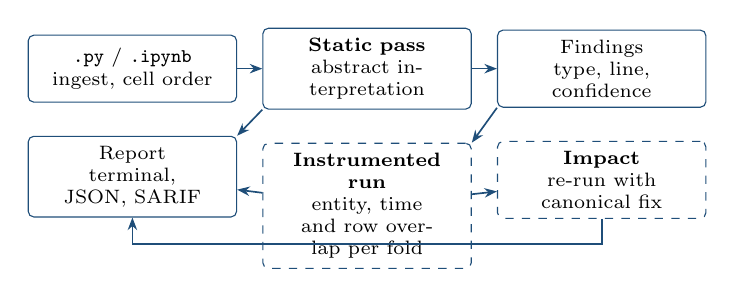
\begin{tikzpicture}[
  node distance=4.2mm and 3.2mm,
  box/.style={draw=navy, rounded corners=2pt, align=center, font=\scriptsize, inner sep=3.5pt, minimum height=8.5mm, text width=24mm, fill=white},
  opt/.style={box, dashed},
  arr/.style={-{Stealth[length=1.6mm]}, navy, semithick}]
\node[box] (in) {\code{.py} / \code{.ipynb}\\ingest, cell order};
\node[box, right=of in] (st) {\textbf{Static pass}\\abstract interpretation};
\node[box, right=of st] (fi) {Findings\\type, line, confidence};
\node[opt, below=of st] (dy) {\textbf{Instrumented run}\\entity, time and row overlap per fold};
\node[opt, below=of fi] (im) {\textbf{Impact}\\re-run with canonical fix};
\node[box, below=of in] (re) {Report\\terminal, JSON, SARIF};
\draw[arr] (in) -- (st);
\draw[arr] (st) -- (fi);
\draw[arr] (fi.south west) -- (dy.north east);
\draw[arr] (dy) -- (im);
\draw[arr] (dy) -- (re);
\draw[arr] (st.south west) -- (re.north east);
\draw[arr] (im.south) -- ++(0,-3.2mm) -| (re.south);
\end{tikzpicture}
\caption{Stages of \tool{}. Dashed stages execute the code and are optional.}
\label{fig:pipeline}
\end{figure}

\subsection{Static pass}

Notebooks are read in execution order when every code cell has a unique execution count, and in cell order
otherwise. One pass of abstract interpretation over the flattened module gives each variable an abstract value:
the origin of a data frame, its known columns, which statistics were computed over which rows, whether rows were
copied or resampled, and the training or evaluation role of a split's result. Rules fire at \emph{sinks}. At a
split point (\code{train\_test\_split}, a splitter's \code{split}, a cross-validation helper, a search object, or
a manual random sample and its complement) it checks for group and temporal leakage and reports statistics or
copied rows that reached the data being split; at a model fit, statistics computed on rows that
include the evaluation side; at a prediction or score, whether the model was fitted on the scored rows; and a
selection over scores computed in a loop gives a multi-test finding.

The evidence for an entity is a column or variable name, or an identifier derived from a file path (for example a
subject code split from a recording's file name). Strong names such as \code{patient}, \code{subject} or
\code{user} can give medium confidence; weak names such as \code{customer}, \code{id} or \code{visit} give low
confidence only. Listing~\ref{lst:example} shows a file-path case.

\begin{lstlisting}[float=t, caption={Group leakage through cross-validation with the default splitter, and the finding the static pass reports for the full file (code and message shortened).}, label={lst:example}, captionpos=b]
recordings = {f"sub-{i:02d}_run-1.npy": ... }
windows, labels, subjects = [], [], []
for fname, signal in recordings.items():
    subject = fname.split("_")[0]
    for w in signal.reshape(-1, 500):
        windows.append([w.mean(), w.std()])
        labels.append(...)
        subjects.append(subject)
X, y = np.array(windows), np.array(labels)
print(cross_val_score(LogisticRegression(), X, y, cv=5).mean())

line 16 [high/medium] group (LL-GRP-003): rows split without regard
  to `subjects`. fix: use GroupKFold with groups=`subjects`
\end{lstlisting}

The analyser prefers missing a leak to inventing one: an unmodelled call depends on all its inputs, and anything
unresolved produces no finding. Loops are analysed once, functions inlined to a fixed depth, and classes are
opaque. pandas, NumPy, scikit-learn~\cite{sklearn} and imbalanced-learn are modelled by name; catalogues and
thresholds are in configuration files.

\subsection{Instrumented run}

Static analysis cannot see an entity column the code never mentions, as when a table with a \code{patient\_id}
column is split at random. The dynamic pass runs the script in a child process with scikit-learn's splitters,
cross-validation helpers, estimator \code{fit}, \code{predict} and \code{score}, and metric functions wrapped.
At each split and fold it records three
facts: rows hashed by value (numbers rounded) on both sides; entity columns, looked up in the row-aligned data
frames of the script's namespace and reported when their values repeat and enough evaluation rows belong to an
entity with training rows; and, for a time column, whether training rows are dated after the earliest evaluation
row. These facts are linked to static findings by call site, so a finding ends up \emph{confirmed},
\emph{refuted} or \emph{not checked}; findings only the run can make, such as duplicate raw records, are added.

\subsection{Impact estimation}

For a located finding, \tool{} re-runs the script with one call site changed. Six fixes are implemented:
duplicated records removed before a split; a row-level split made group-aware on the detected column; a
non-chronological split made chronological; evaluation rows removed from a model fit; a transformer fitted on all
rows refitted on the training rows of a hold-out split; and a feature removed. The estimate is the printed metric
of the original run minus that of the fixed run. Findings without an automatic fix, or whose fixed run fails, are
reported as ``impact unknown'', never dropped; if the fixed run takes a different path, the estimate is marked
unreliable.

\subsection{Running untrusted code, reporting and integration}

Notebooks from the internet run only through a sandbox in an offline cloud session: a child process with an
allow-listed environment, a throwaway working directory, a process-group timeout and an unprivileged user. The
platform (Kaggle) injects session tokens into every job, which a root child could read from \code{/proc}; after
the privilege drop a scan from the child found the token in no ancestor process, a control scan as root in two.

Each finding carries the file, line range, type, rule, confidence, severity, evidence, a suggested fix and, when
measured, the metric before and after the fix, as terminal text, JSON or SARIF (accepted by GitHub code scanning);
a pre-commit hook and a GitHub Action are provided. The tool is deterministic and uses no language model. Of its
373 tests, including property-based tests of termination and determinism, 371 pass on a laptop and the 2 sandbox
tests that need root are skipped (they pass as root in the cloud job).

\section{Benchmark and Evaluation Protocol}

\subsection{Injected benchmark}

No public labelled dataset includes group and temporal leakage, so we built one. Thirteen clean base pipelines
in three families (tabular, time series and grouped data such as multi-visit patients and EEG-style windows) are
mutated by 18 operators. Seventeen inject a leak, for example a scaler fitted before the split or a shuffled
split on time-ordered data. One produces a
\emph{trap}: code that resembles a leak but is correct. Six files combine two leaks. The result is 175 files (94
scripts and 81 notebooks) with 162 labelled leaks, 13 clean files and 6 traps. The lines that carry each leak
are known by construction, and every leaky file has a corrected version, so the true inflation of its metric
can be measured.

Temporal leaks are divided into three categories: \emph{common} (for example an explicit shuffled split),
\emph{differentiating} (cases that pattern-based checks do not cover, such as the default shuffle of
\code{train\_test\_split}) and \emph{hard} (for example a time column with a name that does not suggest time).

The benchmark is split by base pipeline into DEV (7 pipelines, 96 files, 89 leaks) and TEST (6 pipelines, 79
files, 73 leaks). The assignment was committed before any detection rule existed. Rules and thresholds were
tuned on DEV only.

\subsection{Real notebooks}

We sampled 150 public Kaggle notebooks in three query-based strata of 50 and split them by author into DEV (71)
and TEST (79), to be labelled by two people who see no tool output, with Cohen's kappa reported. \textbf{This
labelling has not been done.} On the 71 DEV notebooks the static pass ran without a crash (median 4\,ms per
notebook); without labels, what it flagged is not a result.

\subsection{Protocol}

The protocol was written after DEV results had been seen and frozen before any TEST result existed. A finding
matches a label when it is in the same file and cell, its lines overlap the labelled lines, and its type is the
labelled type or a listed alternative; matching is one-to-one, an unmatched finding is a false positive and an
unmatched label a miss. The operating point is medium or higher confidence. Recall is reported per type with 95\%
percentile bootstrap intervals over files (2,000 resamples). TEST is scored once per release; any later change is
logged and its result labelled a second look. The true inflation of an injected file is the metric of the leaky
file minus that of its corrected version, averaged over five data seeds. The generators were designed, and for
group leakage adjusted after a first measurement, so that each leak type can change the metric; these values
therefore score detection and impact estimates only and are no evidence of severity in practice.

\subsection{Baselines}

\textbf{Yang et al.} We built the released analyser~\cite{yang2022} from source in a Linux cloud job and ran its
default command. Its packaged Datalog engine no longer installs, so the engine was built at version 2.4.1, a
deviation from the released setup; notebooks were given as plain scripts, as its documentation requires. It
reports the affected evaluation line, not the leaking line, so both tools are scored per file and type: a tool is
right about a type in a file when it reports that type and the file has a labelled leak of that type. This rule
was fixed before any baseline output on TEST existed.

\textbf{Data-level and run-time tools.} leakcheck-ml~\cite{leakcheckml}, LeakHound~\cite{leakhound},
dataleaks~\cite{dataleaks} and Deepchecks~\cite{chorev2022} take a training and a test table, not code. The
instrumented run of \tool{} exports, at every split call and for up to five folds, the tables the pipeline used
(every row-aligned column, the label column removed and the target kept apart). Each tool received every pair with
its defaults and again with the true entity or time column named through its own parameter; a detection is placed
at the split call's line. splitguard~\cite{splitguard} instruments a run itself and was run as documented and with
the true group declared through \code{mark\_groups}. Each tool ran at the cited version in its own environment, one
finding per file, line and type, after the single TEST run of \tool{}.

\textbf{Not run.} scicode-lint~\cite{samsonau2026} needs a GPU with at least 16\,GB and native FP8 support. On two
NVIDIA T4 GPUs (no FP8) its pinned server (vLLM~0.18.0) failed to start, and a fallback (llama.cpp, same model at
8 bits) produced no result within 20 minutes for any of the 29 files it attempted; it is reported as not run, not
as zero. LeakCheck~\cite{draoui2026} needs a paid LLM interface and an access-restricted package.

\section{Results}

\subsection{Detection on the held-out split}

Table~\ref{tab:test} gives the single TEST run: 59 of 73 leaks found statically (0.81) and 65 with the run (0.89),
no false positive in either mode, and no finding on the 9 leak-free files. The run confirmed 43 static findings,
refuted none, could not check 25 (no run-time check exists for forward-looking features or pandas statistics) and
added 2, both duplicated records. By temporal category the tool found 5 of 5 common, 7 of 7 differentiating and 8
of 13 hard leaks. On DEV, where the rules were tuned, it found 80 of 89 statically and 89 of 89 with the run; the
drop from DEV to TEST is real.

\begin{table}[t]
\caption{Detection on the injected TEST split (79 files, 73 leaks), scored once. Findings of medium or higher
confidence. Recall with 95\% bootstrap interval over files. No false positive in either mode.}
\label{tab:test}
\footnotesize
\setlength{\tabcolsep}{2.6pt}
\begin{tabular}{@{}lrrlrl@{}}
\toprule
 & & \multicolumn{2}{c}{\textbf{Static}} & \multicolumn{2}{c}{\textbf{Static + run}} \\
\cmidrule(lr){3-4}\cmidrule(l){5-6}
\textbf{Type} & \textbf{Leaks} & \textbf{Found} & \textbf{Recall} & \textbf{Found} & \textbf{Recall} \\
\midrule
Preprocessing & 22 & 21 & 0.95 (0.84--1.00) & 21 & 0.95 (0.84--1.00) \\
Overlap & 9 & 7 & 0.78 (0.44--1.00) & 9 & 1.00 (1.00--1.00) \\
Multi-test & 6 & 5 & 0.83 (0.43--1.00) & 5 & 0.83 (0.43--1.00) \\
Group & 7 & 3 & 0.43 (0.00--0.83) & 7$^{*}$ & 1.00$^{*}$ \\
Temporal & 25 & 20 & 0.80 (0.62--0.95) & 20 & 0.80 (0.62--0.95) \\
Target-derived & 4 & 3 & 0.75 (0.00--1.00) & 3 & 0.75 (0.00--1.00) \\
\midrule
All types & 73 & 59 & 0.81 & 65 & 0.89 \\
\bottomrule
\end{tabular}

\vspace{2pt}
\raggedright $^{*}$By the matching rule, which checks type and line. Only 3 of the 7 findings name the true
entity column, so the strict figure is 0.43.
\end{table}

\subsection{What went wrong on TEST, and a second look}

\textbf{Right line, wrong column.} In a patient-visits pipeline the static pass guessed, at low confidence, a
column named \code{visit}; the run checked only nominated columns, found visit numbers on both sides of the split,
as always, and raised the confidence without examining \code{patient\_id}. The matching rule ignores the column,
so Table~\ref{tab:test} counts these four findings as correct; they are not, nor is their impact estimate. \textbf{A slice mistaken for a split.} A pipeline dropping
its last row with \code{data.iloc[:-1]} was read as the training side of a manual split: five temporal leaks
were reported at low confidence only and one multi-test leak was missed. \textbf{An unresolved column filter.} A
feature list built with a \code{startswith} filter could not be resolved, so two leaks were not reported.

The three faults were then fixed and logged. DEV was unchanged, and TEST gave 67 of 73 statically and 73 of 73
with the run, with no false positive; the patient findings now name \code{patient\_id},
and the EEG ones a run-time variable holding the subject identifiers. The fixes were written knowing which TEST
files they repair, so this is not a held-out result and Table~\ref{tab:test} remains the result of record. The
injected benchmark is now saturated on both halves.

\subsection{Comparison with Yang et al.\ on the same files}

On the three types the baseline supports (Table~\ref{tab:yang}), it found 20 of 37 files with one false alarm, and
the static pass of \tool{} 33 of 37 with none; both analysed all 79 files and reported nothing on the leak-free
ones. On the 37 file-and-type pairs \tool{} alone was right in 14, the baseline alone in 1, both in 19 and neither
in 3 (exact McNemar test, $p<0.001$). The difference comes from preprocessing (12 against 1); on overlap the tools
agree on every file. The comparison favours \tool{}: neither tool was tuned on these files, but they were
generated by our operators, with the kinds of leak \tool{} was built for.

\begin{table}[t]
\caption{Yang et al.\ and \tool{} (static mode) on the 79 injected TEST files, scored per file and type.
``Found'': files with this leak in which the tool reports the type. ``False'': files where it reports the type
wrongly.}
\label{tab:yang}
\footnotesize
\setlength{\tabcolsep}{4.5pt}
\begin{tabular}{@{}lrrrrr@{}}
\toprule
 & & \multicolumn{2}{c}{\textbf{Yang et al.~\cite{yang2022}}} & \multicolumn{2}{c}{\textbf{\tool{} (static)}} \\
\cmidrule(lr){3-4}\cmidrule(l){5-6}
\textbf{Leakage type} & \textbf{Files} & \textbf{Found} & \textbf{False} & \textbf{Found} & \textbf{False} \\
\midrule
Preprocessing & 22 & 10 & 1 & 21 & 0 \\
Overlap / duplicates & 9 & 7 & 0 & 7 & 0 \\
Multi-test & 6 & 3 & 0 & 5 & 0 \\
\midrule
Group$^{\dagger}$ & 7 & 0 & 0 & 3 & 0 \\
Temporal$^{\dagger}$ & 24 & 3 & 0 & 19 & 0 \\
Target-derived$^{\dagger}$ & 4 & 0 & 0 & 3 & 0 \\
\bottomrule
\end{tabular}


\vspace{2pt}
\raggedright $^{\dagger}$Not a type the baseline claims to detect. It is credited under temporal in 3 files where
it reports whole-series scaling as preprocessing leakage. Temporal has 24 files for 25 leaks because one file
holds two.
\end{table}

\subsection{Leaks at a split: data-level and run-time tools}

Table~\ref{tab:baselines} covers the TEST leaks at a split call, the only ones a data-level tool can see: 8
non-chronological splits of time-ordered data, 7 group splits and 2 sets of duplicated raw records. Without a
named column, leakcheck-ml finds 4 of 7 group splits, all with the right column, and 3 of 8 time splits;
LeakHound, Deepchecks and splitguard find none of either. With the column named, leakcheck-ml and LeakHound find
7 of 8 and 7 of 7. dataleaks finds 7 of 7 group splits without a hint, but names an unrelated column in 3, flags 2
of the 9 leak-free files and has no split-order check by default. Deepchecks has no group check; splitguard needs
the group declared and misses the held-out rows of \code{next(splitter.split(...))}. All data-level tools find
the duplicated records. \tool{} finds 8 of 8 time splits with no column named, but only 3 of its 7 group findings
name the true entity, against 4 for leakcheck-ml without a hint. The other tools also need exported tables,
which our run supplied here.

\begin{table}[t]
\caption{Leaks at a split call, injected TEST (\tool{}: first look). Col.: true entity or time column named to
the tool. T1: non-chronological splits of time-ordered data. Grp: group splits (matching rule); Grp, col.: those
naming the true entity. Dup.: duplicated raw records. Clean: leak-free files with any finding.}
\label{tab:baselines}
\footnotesize
\setlength{\tabcolsep}{2.6pt}
\begin{tabular}{@{}llrrrrr@{}}
\toprule
\textbf{Tool} & \textbf{Col.} & \textbf{T1} & \textbf{Grp} & \textbf{Grp, col.} & \textbf{Dup.} & \textbf{Clean} \\
 & & /8 & /7 & /7 & /2 & /9 \\
\midrule
\tool{} (static + run) & no & 8 & 7 & 3 & 2 & 0 \\
\midrule
leakcheck-ml & no & 3 & 4 & 4 & 2 & 0 \\
 & yes & 7 & 7 & 7 & 2 & 0 \\
LeakHound & no & 0 & 0 & 0 & 2 & 0 \\
 & yes & 7 & 7 & 7 & 2 & 0 \\
dataleaks & no & 0 & 7 & 4 & 2 & 2 \\
 & yes & 0 & 7 & 7 & 2 & 2 \\
Deepchecks & no & 0 & 0 & 0 & 2 & 0 \\
 & yes & 7 & 0 & 0 & 2 & 0 \\
splitguard & no & 0 & 0 & 0 & 0 & 0 \\
 & yes & 0 & 7 & 7 & 0 & 0 \\
\bottomrule
\end{tabular}

\end{table}

\subsection{Impact estimates}

On TEST an estimate could be produced for 34 of 70 located leaks (group 7 of 7, target-derived 3 of 3, overlap 7
of 9, preprocessing 10 of 21, temporal 7 of 25, multi-test 0 of 5); the rest are reported as unknown with the
reason. The instrumented script printed exactly the plain script's metric in all 395 runs. For 26 single-leak
findings with a bounded metric, averaged over five seeds, the mean absolute error against the true inflation was
0.035 and the rank correlation 0.58. The estimate was exact where our fix is the same operation as the
benchmark's corrected file, a weak test, and wrong in direction for hold-out group splits ($-0.084$ against a
true $+0.212$ AUC) because the fix grouped by the wrong column. In the second look the error was 0.0006 and the
correlation 0.97, with the same caveat as for detection.

LeakHound (Table~\ref{tab:impact}) compares its own model on the exported split with a group-aware or
chronological split it builds. Where both tools gave an estimate (11 findings), LeakHound's mean absolute error was 0.065 and \tool{}'s
0.086: \tool{} was worse on the hold-out group splits, where it grouped by the wrong column, and exact on
duplicated records and time splits, where LeakHound was off by 0.01 to 0.08. With the column fault repaired
(second look, not held out) \tool{}'s error on the same 11 findings was 0.020. LeakHound gave no estimate for
preprocessing or target-derived findings, and none without a named column except for duplicated records. The
near-zero preprocessing errors carry little information, as those leaks barely inflate the metric.

\begin{table}[t]
\caption{Impact estimates against the true inflation, injected TEST, single-leak files, seed 0 (\tool{}: first
look). N: findings. Comp.: pipelines reporting AUC or $R^2$, LeakHound's metrics. Cells: estimates (mean absolute
error). LH: LeakHound with defaults; LH, col.: with the true column named.}
\label{tab:impact}
\footnotesize
\setlength{\tabcolsep}{2.4pt}
\begin{tabular}{@{}lrrlll@{}}
\toprule
\textbf{Type} & \textbf{N} & \textbf{Comp.} & \textbf{\tool{}} & \textbf{LH} & \textbf{LH, col.} \\
\midrule
group & 6 & 6 & 6 (0.158) & 0 (--) & 6 (0.075) \\
overlap & 6 & 6 & 6 (0.000) & 2 (0.043) & 2 (0.043) \\
preproc. & 8 & 8 & 8 (0.000) & 0 (--) & 0 (--) \\
target-der. & 3 & 3 & 3 (0.000) & 0 (--) & 0 (--) \\
temporal & 6 & 3 & 3 (0.000) & 0 (--) & 3 (0.059) \\
\bottomrule
\end{tabular}

\end{table}

\subsection{Running time and a negative case study}

The static pass took a median of 2.6\,ms per file and the instrumented run 1.3\,s (maximum 12.7\,s) on a laptop;
the Yang analyser took a median of 6.2\,s per file in a cloud CPU job (different machines, so
scale only).

We also ran the static pass on a separate EEG seizure-detection codebase by the first author, with three
evaluation regimes of known leakage status: random windows, a within-patient split and leave-one-patient-out. It
reported nothing in the 78 files: correct for the third regime, a miss for the first two. The code splits
with hand-written NumPy masks and by position over lists of custom objects, with subject identity an object
attribute: there is no splitter, data frame or column name to model, for either pass. No rule was changed after this result.

\section{Limitations and Threats to Validity}

\textbf{No result on real code.} The tool and the injected benchmark share authors, and TEST uses different
pipelines but the same mutation operators as DEV, so the results measure generalisation across pipelines, not
across the ways people write leaks; a precision of 1.00 on short synthetic files will not hold on real notebooks. \textbf{Small samples.} TEST has 4 target-derived, 6 multi-test
and 7 group leaks. \textbf{Blindness.} The column names of the TEST pipelines were seen by
mistake while rules were written; no TEST code, label or operator was read, but TEST group results are not blind
to entity names. \textbf{Heuristic entity inference.} Evidence for an entity is a name, repetition or a file path;
a name can mislead in both directions, as the first TEST run shows. \textbf{Coverage of code styles.} Hand-written
splits, custom classes and deep learning frameworks are largely outside the analysis, as the case study shows.
\textbf{Impact estimates.} Automatic fixes cover six situations, about half of the located leaks; a group-aware or chronological split changes which rows are
evaluated, so an estimate is the change under the canonical fix, not a causal decomposition.
\textbf{Baselines.} The Yang analyser was scored under a looser rule than the protocol's; the data-level tools
used tables exported by our run; scicode-lint and LeakCheck could not be run.

\section{Conclusion and Future Work}

\tool{} detects six leakage types in Python ML code, including group leakage from source code, links static
findings to an instrumented run, and measures a located leak's effect by re-running the pipeline with a fix. On
held-out injected leaks it found 81\% of leaks statically and 89\% with the run, with no false positive, more
than the reference static analyser ($p<0.001$), and alone found time-order leaks with no column named. On group
leaks, tools told the entity column matched or beat it, and a confirmation fault named the wrong entity in four of
seven findings; hand-written splits are invisible to it.

Next, labelling the 150 sampled notebooks will test these results on real code; we also plan to run scicode-lint
on FP8 hardware, cover manual and framework-specific splits, and measure the prevalence and impact of each leakage
type in public notebooks.

\textbf{Data and code availability.} The code, benchmark generators, frozen protocol, change log and the output
of every cited run are released under the MIT licence at
\url{https://github.com/bytes06runner/LeakLens}.

\section*{Acknowledgment}

The implementation was written with the help of an AI coding assistant; the authors made the design and
protocol decisions and reviewed all reported results.

\bibliographystyle{IEEEtran}
\bibliography{references}

\end{document}
